


\section{SourceForge}

\begin{figure}[h]
\centering
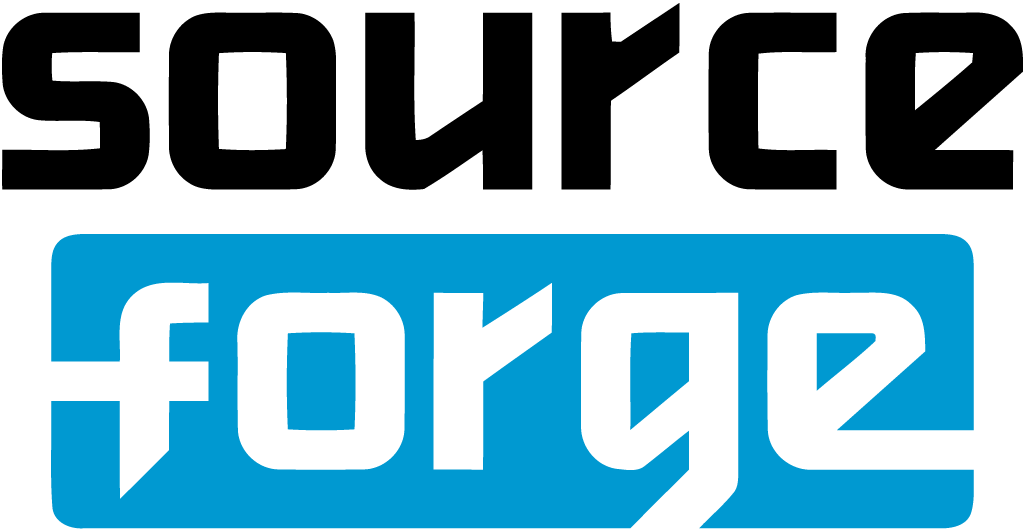
\includegraphics[width=0.4\linewidth]{sourceforge-logo}
\end{figure}

\subsection{Allgemeines}

SourceForge ist eigentlich ein englisches Wort und bedeutet soviel wie \glqq Quellentextschmiede\grqq. Es ist ein Repository in Form einer Website. Mit SourceForge ist es möglich Softwareprojekte online zu erstellen und zu verwalten. Was dabei zu beachten ist, ist, dass eine Registrierung optional ist. Dass bedeutet, man kann öffentliche Projekte auch ohne einen Account einsehen. SourceForge wird betrieben vom US-amerikanischen Unternehmen \glqq Dice Holdings\grqq. Au{\ss}erdem war es bis zur Version 3 eine freie Software, wurde daraufhin allerdings proprietär und kommerziell vertrieben. Viele bekannte Open Source Projekte sind auf SourceForge vertreten, wie zum Beispiel Hibernate, Moodle oder auch FileZilla. Des Weiteren bietet SourceForge im Gegensatz zu vielen Konkurrenten, mehr als nur ein System zur Versionsverwaltung an. 

Dazu zählen: 
\begin{itemize}
	\item CVS
	\item SVN
	\item Bazaar
	\item Git
	\item Mercurial
\end{itemize}
\noindent
SourceForge wird von vielen Software Entwicklern genutzt, weil es neben der Hauptaufgabe als Online-Repository noch weitere Vorteile bietet. Beispielsweise kann jedes Projekt über ein eigenes Wiki verfügen, in dem wichtige Informationen über das Projekt aufgelistet sind. Ein anderer Punkt ist, dass SourceForge für jedes einzelne Projekt auch die Möglichkeit bietet, auf eine eigene MySQL-Datenbank zuzugreifen.

\subsection{Einschränkungen}
Der Zugriff auf SourceForge wurde vor einiger Zeit in China gesperrt, aufgrund des Projektes \glqq Goldener Schild\grqq \space. Das soll eine Anlehnung an die Chinesische Mauer sein. Dieses Projekt ist für die überwachung der Zensur im chinesischen Internetverkehr zuständig. Allerdings wurde diese Sperrung nach bereits einem Jahr wieder aufgehoben. 2008 wurde der Zugang aber wieder gesperrt, weil vermutet wird, dass sich ein SourceForge-Programmierer negativ über die chinesische Regierung geäu{\ss}ert hat. 

Des Weiteren wurde SourceForge in einigen sogenannten \glqq Schurkenstaaten\grqq \space gesperrt. Das sind Staaten, die auf der Sanktionsliste der USA sind. Einige betroffene Länder sind Nordkorea, Syrien, Sudan und Kuba. Aufgrund der Reaktion der Community wurde diese Einschränkung aber ein wenig gelockert. Es ist nun möglich, dass der Administrator jedes Projektes selbst bestimmen kann, ob er den Zugang zum Projekt in diesen Ländern freigeben möchte. 

\subsection{Kritikpunkte}
In letzter Zeit wurde SourceForge stark kritisiert, weil sie auf sogenannte \glqq Drive-By-Installer\grqq \space zurückgriffen. Diese sorgen dafür, dass bei der Installation von SourceForge weitere Installationen von Adware von Drittanbietern vorgeschlagen wird. Ein Beispiel für eine solche Adware ist die \glqq Ask-Toolbar\grqq. Das ganze wurde wahrscheinlich gemacht, um an zusätzliches Geld zu kommen, allerdings war die Community damit nicht zufrieden und deswegen hat SourceForge in letzter Zeit stark an aktiven Mitgliedern verloren. 

\subsection{ähnliche Projekte}

SourceForge war eine Art Vorreiter auf dem Gebiet von Online-Repositories. Heute gibt es allerdings jede Menge Konkurrenten, die teilweise auch schon erfolgreicher sind als SourceForge. Dazu zählt Github, ein Online-Repository, dass mit dem Versionsverwaltungssystem Git arbeitet. Weitere Beispiele sind Bitbucket, dass Mercurial zur Versionsverwaltung benutzt, Codeplex, was eine Hosting Website von Microsoft für Open Source Projekte ist und Freecode, ein Katalog für Open Source Projekte.


